\section{Results}



\subsection{Proportional Increase}
%\subsection{VAR(4) Model}
%
%Figure~\ref{fig:results_simplevar} shows the forecasts for the different scenarios in the case of the VAR(4) model in levels\footnote{[Review Comment:] Should I also report the confidence intervals (95\%) of the different forecasts here? Also, a more general question: The confidence intervals of the different forecasts overlap to some extent. The question now is what this tells me about the about the significance of the effects. If I run into problems here, I'd love some advice on how to deal with that problem.}. Table~\ref{tab:peak_simple} also shows the peak effects, which were calculated as the difference between the scenario forecast and the baseline forecast divided by the baseline value of the same period. As the forecasts originate from the same data in our presample period prior to 2013 Q2, the two scenarios differ only in their effect size, but not in their qualitative interpretation. Accordingly, replacing the increase in government spending by a decrease results in a mirrored image of the corresponding effects.
%
%For GDP, an increase in government spending causes an instant effect in the first period, which constitutes the peak impact of 1.30\% in the first scenario and 3.26\% in the second scenario. Sustaining these higher levels of spending, however, result in a slight decrease after one quarter and a reversal after the third quarter, where the values of GDP lie constantly below the baseline. Only after seven quarters, we can again observe a slight increase, but the original baseline levels are not reached in either scenario after two years.
%
%We can observe similar patterns for the excess stock returns of the construction sector and CPI inflation. Similarly to GDP, inflation increases after one quarter, reaching its peak effect of 0.16 percentage points in scenario 1 and 0.39 percentage points in scenario two. After five quarters, inflation falls below the baseline and stabilizes below the baseline. In the case of the excess stock returns, there is a longer lasting positive impact, and we reach a peak after one year of 18.12 percentage points and 45.30 percentage points respectively. Then, however, we find a reversal, where the excess stock returns decrease and fall below baseline levels after seven quarters. In contrast to GDP and inflation, excess stock returns also continue decreasing until the end of two years.
%
%Consumption and investment, on the other hand, exhibit clearer tendencies without a clear reversal within two years. Consumption increases from the first quarter onwards, reaching its peak effect of 1.47\% or 3.81\% after five quarters, and outperforms the baseline for the whole forecast period. The effects on investment, however, are even more pronounced. From the first period onwards, the increase in government spending leads to a drastic decrease of investment over the whole period, indicating a crowding out of private investment caused by the sustained higher levels of government spending. The peak effects on investment, indicating a decrease of 17.29\% and 43.22\% are the largest deviation from the baseline in our set of endogenous variables.
%
%
%
%\begin{figure}[ht]
%	\centering
%		\includegraphics[scale=0.55]{scenarios_simplevar_setting1.jpg}
%	\caption{Scenario forecasts for the VAR(4) model.}
%	\label{fig:results_simplevar}
%\end{figure}
%
%
%\begin{table}[ht]
%\centering
%%\begin{adjustbox}{width=1\textwidth}
%\begin{tabular}{|p{3cm}|p{1cm}|p{1.8cm}|p{1.6cm}|p{2.2cm}|p{1.6cm}|}
%\hline
%  & GDP    & Investment & Excess Stock Returns &	Consumption & CPI Inflation \\ \hline \hline
%Scenario 1 - +10 \%                   & 1.30\% & -17.29\%   & 18.12 pp             & 1.47\%      & 0.16 pp       \\
%\hline
%Scenario 2 - +25 \%                   & 3.26\% & -43.22\%   & 45.30 pp             & 3.81\%      & 0.39 pp    \\
%\hline  
%\end{tabular}
%
%%\end{adjustbox}
%\caption{Peak Effects in the VAR(4) forecasts.}
%\label{tab:peak_simple}
%\end{table}

%\subsection{dVAR(3) Model}


As Table~\ref{tab:wtest} shows for the shift in government spending, only the policy forecasts for GDP and Consumption growth differ significantly from the baseline forecast. We would hence conclude, that, in the median, a constant increase in government spending only has a significant effect on those two variables. The 8-step forecasts estimated for all series from the model can be seen in Figure~\ref{fig:results_dvar}. These results described above persist en gros after increasing the number of exogenous lags in government expenditure, except for a significant - but nonetheless similarly small - effect size on CPI for $q \geq 3$. 

For GDP growth, the increase in government spending in the second quarter of 2013 let to an instant shift in both scenarios. Thereafter, the paths for the counterfactual scenarios are simply shifted and diverge increasingly with time. In any case, however, both the difference between the scenarios and the speed of their divergence are very small with a peak effect of 0.05 percentage points in 2015 Q2 for Scenario 1, and a peak effect of 0.13 percentage points for Scenario 2 in 2015 Q2. The growth paths for consumption develop in a similar fashion as for GDP. In both scenarios, the forecasts stay relatively close to the baseline and then reach their respective peak effects at the end of the forecast horizon at 0.05 percentage points and 0.12 percentage points in 2015 Q2.

Given the relatively strong assumption of the policy scenarios, in which the policymakers could raise government spending 10\% and 25\% higher than they actually did, the effects of the policy change are surprisingly small. Even more so, as the effect seemed to not manifest itself across all the variables we were considering in this exercise.

\begin{figure}[!htbp]
	\centering
	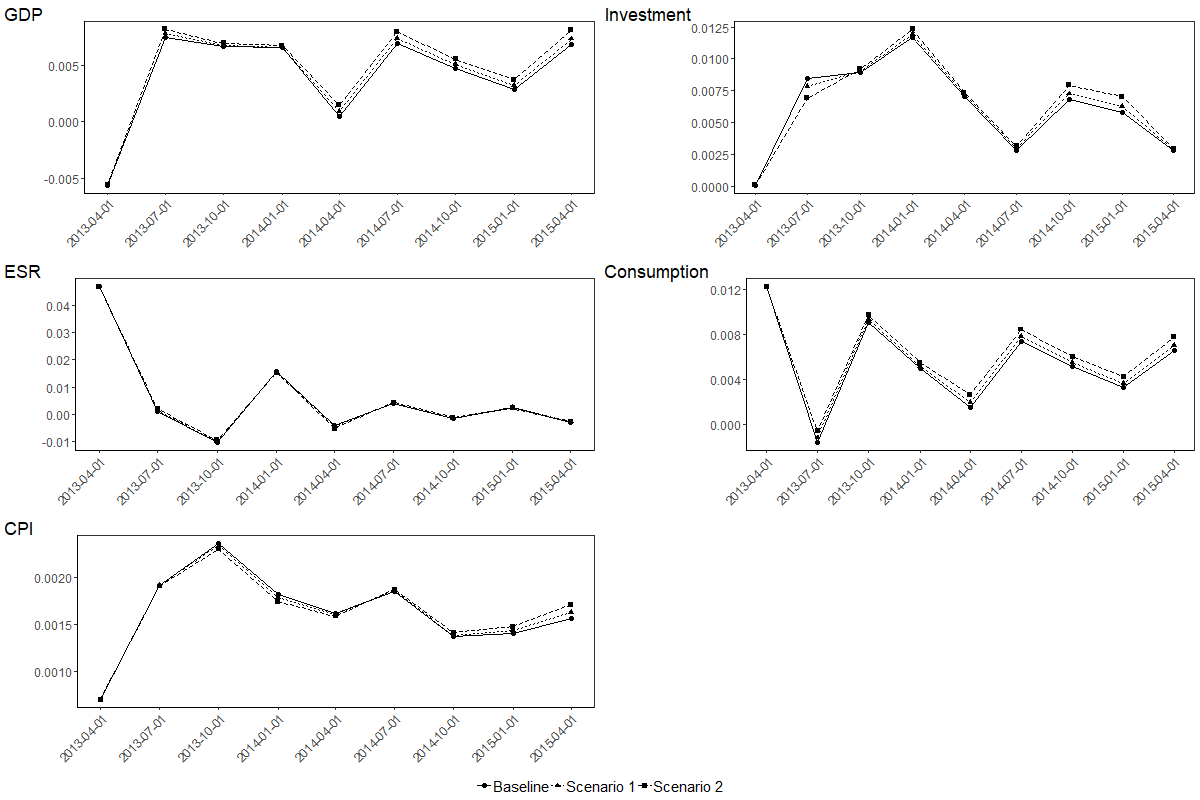
\includegraphics[width=1\textwidth,height=1\textheight,keepaspectratio]{scenariofcst.png}
	\caption{Forecasts for the policy scenarios with a proportional increase over the forecast horizon.}
	\label{fig:results_dvar}
\end{figure} 

\begin{table}[!htbp] \centering 
	\caption{Peak effects and results of Wilcoxon Signed Rank test for the scenarios vs. baseline for a proportional increase over the forecast horizon} 
	\label{tab:wtest} 
	\begin{tabular}{@{\extracolsep{5pt}} lrrrr} 
		\\[-1.8ex]\hline 
		\hline \\[-1.8ex]
		& Peak Effect 10\% & Peak Effect 25\% & Test Statistic & p \\ 
		\hline \\[-1.8ex] 
		GDP & $0.05$ p.p. & $0.13$ p.p. & $0$ & $0.01$ \\ 
		Investment & $-0.06$ p.p. & $-0.15$ p.p. & $8$ & $0.20$ \\ 
		ESR & $0.05$ p.p. & $0.12$ p.p. & $16$ & $0.84$ \\ 
		Consumption & $0.05$ p.p. & $0.12$ p.p. & $0$ & $0.01$ \\ 
		CPI & $0.006$ p.p. & $0.01$ p.p. & $16$ & $0.84$ \\ 
		\hline \\[-1.8ex] 
	\end{tabular} 
\end{table}  

%\begin{table}[!htbp] \centering 
%	\caption{Jarque-Bera Test Statistics for the dVar(3) Model} 
%	\label{tab:jbtest} 
%	\begin{tabular}{@{\extracolsep{5pt}} cc} 
%		\\[-1.8ex]\hline 
%		\hline \\[-1.8ex] 
%		Statistic & p  \\ 
%		\hline \\[-1.8ex] 
%		$94.2727$ & $0.000$ \\ 
%		\hline \\[-1.8ex] 
%	\end{tabular} 
%\end{table}


\subsection{Constant Increase}

Figure~\ref{fig:results_dvarL} shows the forecasts with a constant increase in government spending in each period of the forecast horizon. Notably, the differences in the growth paths of the variables between the baseline forecast and the alternative policy scenarios are more pronounced than during a period of proportionally increased government spending. For GDP and ESR and consumption the forecasts indicate an increase in growth right from the beginning, followed by a decrease below baseline levels and consequent convergence where consumption growth converges the latest toward the baseline. The deviations are more pronounced for Scenario 2 than they are for Scenario 1. Investment growth exhibits fluctuations in the opposite direction as the other variables.. The only statistically significant effect after the increase is seen in inflation, reaching its peak effects 0.62 and 1.54 percentage points in the respective scenario. It is also the only variable that still shows a relatively clear difference between the scenarios and the baseline at the end of the forecast horizon.

Although the total size of the increase over the forecast horizon is the same as for the proportional spending increase, the effects exhibited in the forecasts, both in terms of behavior over time and statistical significance are quite different. The differences in the variables other than inflation seem to whither away over time, leaving the economy with temporarily increased inflation, which is also drifting back to its pre-policy levels. 

\begin{figure}[!htbp]
	\centering
	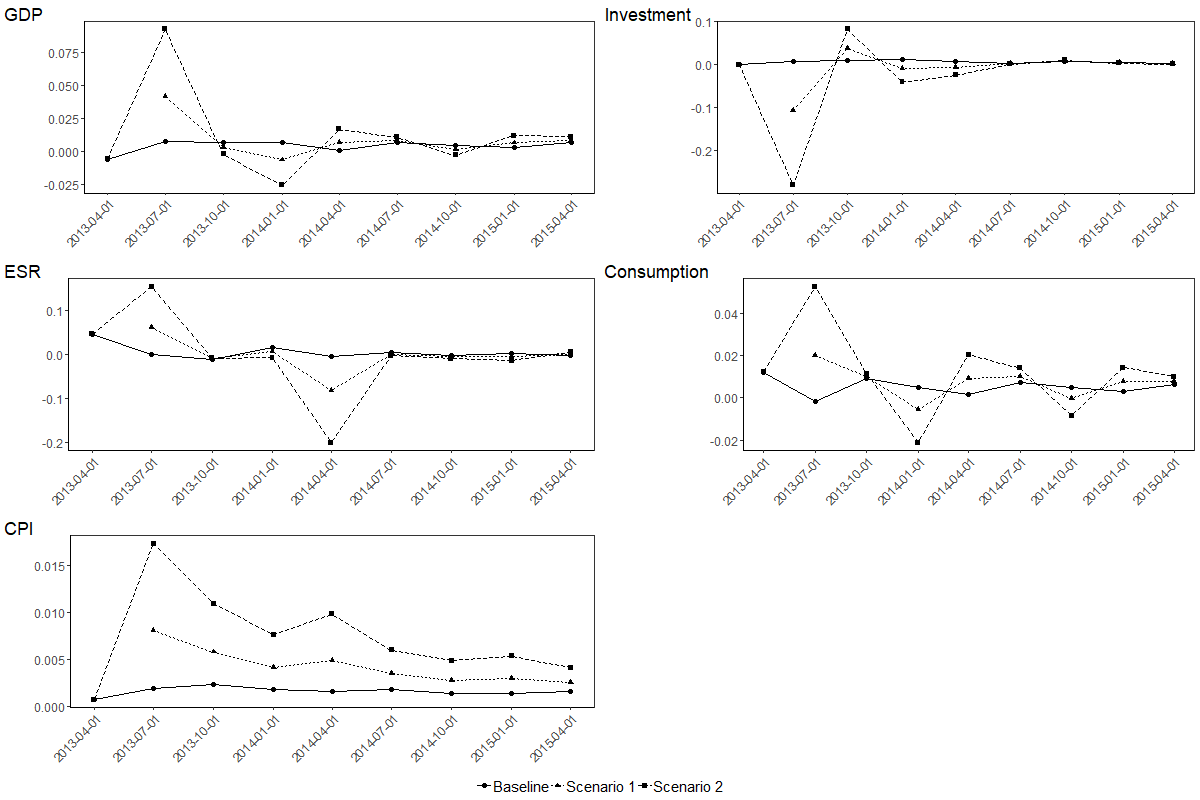
\includegraphics[width=1\textwidth,height=1\textheight,keepaspectratio]{scenariofcst_linear.png}
	\caption{Forecasts for the policy scenarios for a constant increase over the forecast horizon.}
	\label{fig:results_dvarL}
\end{figure} 

\begin{table}[!htbp] \centering 
	\caption{Peak effects and results of Wilcoxon signed-rank test of the scenarios vs baseline for a constant increase over the forecast horizon.} 
	\label{tab:wtestL} 
	\begin{tabular}{@{\extracolsep{5pt}} lrrrr} 
		\\[-1.8ex]\hline 
		\hline \\[-1.8ex]
		& Peak Effect 10\% & Peak Effect 25\% & Test Statistic & p \\ 
		\hline \\[-1.8ex] 
		\hline \\[-1.8ex] 
		GDP & $3.40$ p.p. & $8.50$ p.p. & $14$ & $0.64$ \\ 
		Investment & $-11.58$ p.p. & $-28.95$ p.p. & $25$ & $0.38$ \\ 
		ESR & $-7.84$ p.p. & $-19.60$ p.p. & $24$ & $0.46$ \\ 
		Consumption & $2.18$ p.p. & $5.46$ p.p. & $12$ & $0.46$ \\ 
		CPI & $0.62$ p.p. & $1.54$ p.p. & $0$ & $0.01$ \\ 
		\hline \\[-1.8ex] 
	\end{tabular} 
\end{table}  

\subsection{One-Time Increase with Instant "Payback"}

Directionally, the responses in GDP and investment growth after a unique increase of government spending in the first quarter of the forecast horizon are similar to the responses after a constant spending increase, albeit with their peaks shifted to the first quarter after the increase happens. Consumption growth also shows a pattern of fluctuation similar to the one in the constant spending increase scenario. ESR growth fluctuates away from the baseline much more clearly in this scenario than before, falling beneath base levels six months after the increase and remains lower than the baseline until it recovers and then comes back to baseline levels. Inflation is - like the other variables - also not significantly affected by the policy measure, converging to the baseline quickly. The effects remain unsignificant even after doubling the increases in the respective scenarios, indicating that the effects of one-off increases in government expenditure are rather scale-insensitive and do not affect the growth paths of the variables in question.

\begin{figure}[!htbp]
	\centering
	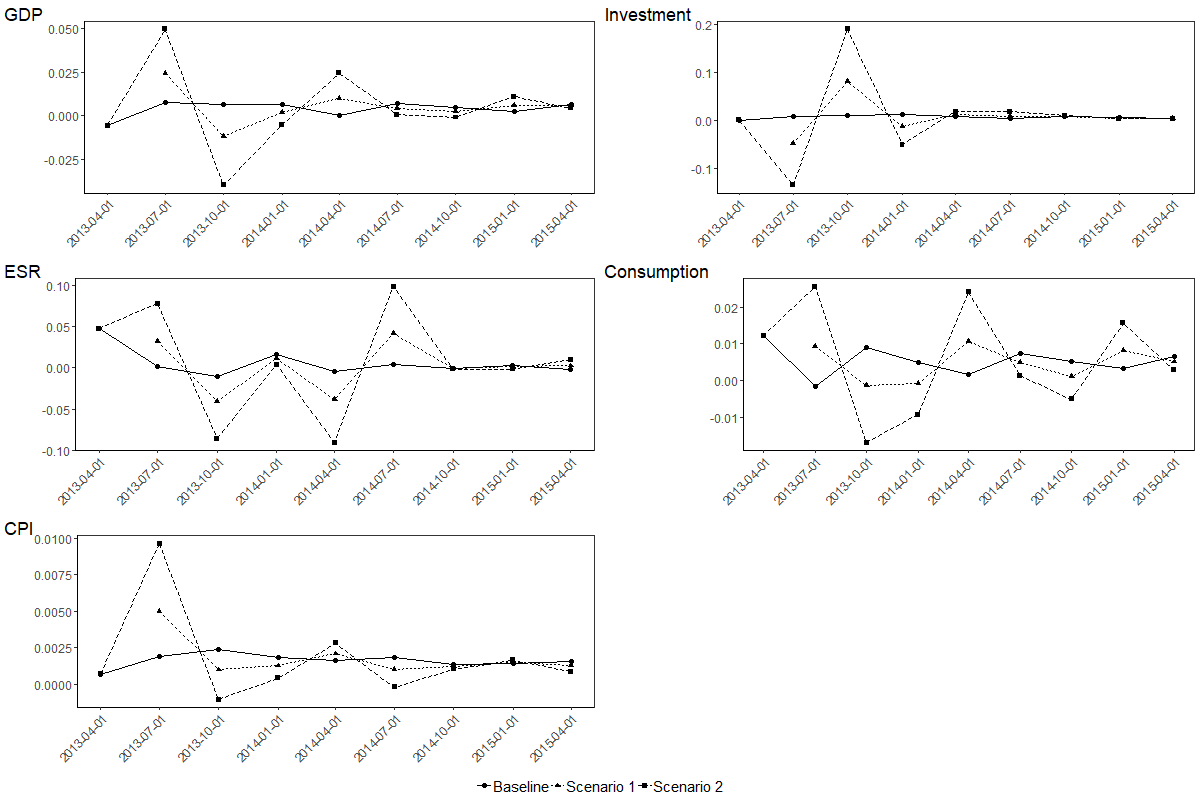
\includegraphics[width=1\textwidth,height=1\textheight,keepaspectratio]{scenariofcst_OneTime.png}
	\caption{Peak effects and results of Wilcoxon signed-rank test of the scenarios vs baseline for a one-time increase.}
	\label{fig:results_dvarOT}
\end{figure} 

\begin{table}[!htbp] \centering 
	\caption{Results of Wilcoxon Signed Rank test for Scenarios vs Baseline for a one-time increase.} 
	\label{tab:wtestOT} 
	\begin{tabular}{@{\extracolsep{5pt}} lrrrr} 
		\\[-1.8ex]\hline 
		\hline \\[-1.8ex]
		& Peak Effect 10\% & Peak Effect 25\% & Test Statistic & p \\ 
		\hline \\[-1.8ex] 
	\hline \\[-1.8ex] 
	GDP & $-1.86$ p.p. & $-4.66$ p.p. & $19$ & $0.95$ \\ 
	Investment & $7.26$ p.p & $18.07$ p.p. & $16$ & $0.84$ \\ 
	ESR & $3.76$ p.p. & $9.41$ p.p. & $18$ & $1.00$ \\ 
	Consumption & $1.09$ p.p. & $2.72$ p.p. & $18$ & $1.00$ \\ 
	CPI & $0.31$ p.p. & $0.77$ p.p. & $23$ & $0.55$ \\ 
	\hline \\[-1.8ex] 
	\end{tabular} 
\end{table}  


%The effect sizes are similarly small for investment growth, but the behavior of the growth paths, is more interesting. In the first period, the increase in government spending seems to slightly slow down investment growth. The picture reverts, however, as in both scenarios investment growths jumps ahead of the baseline from the second quarter after the increase onwards. Both scenarios again reach their peak effect at the same time in the first quarter of 2015 with 0.04 percentage points in Scenario 1 and 0.12 percentage points in Scenario 2. In the last period, all forecasts converge again.



%The effects of an increase in government spending on the growth path of GDP are less straightforward than the level effects we obtained from the VAR(4) model. Upon increasing government expenditure, GDP growth reaches a peak effect of 1.59 percentage points in the first, and 3.98 percentage points in the second scenario. After that, however, the sustained levels of government expenditure cause GDP growth to fall below the baseline in the second and third quarter, after which it returns to a similar growth path as in the baseline scenario. In our forecasts we can observe similar patterns for the growth paths of investment and consumption. The growth of consumption increases in the first quarter by 0.98 or 2.44 percentage points, respectively, after which it fluctuates around the growth path of the baseline prediction. Furthermore, the higher levels of government expenditure seem to intensify the volatility of consumption growth. For investment growth, the increase in government expenditure here also has a negative effect. It is, however, less persisting than in the VAR(4), case. Right after the increase of government expenditure, the growth rate for investment drops by 5.87 percentage points in scenario 1 and 14.68 percentage points in scenario two. Then, however, the growth rate stabilizes around the baseline after five quarters, indicating quite a different effect in levels compared to the VAR(4) model.
%
%Similarly interesting are the effects of the increase in government spending on excess stock returns and CPI inflation. As mentioned above, these time series were not modified for the dVAR(3) model, as they were already expressed as logarithmic differences. The implications of the dVar model, however, seem to have quite different implications on these series. In the case of the excess stock returns, the increase in government expenditure causes them to increase for the first three quarters by up to 9.96 percentage points and 24.91 percentage points. Then, after the third quarter, they approach the levels of the baseline forecast without reaching them within two years, however. In the first quarter, CPI inflation also increases by 0.29 percentage points in scenario 1 and 0.72 percentage points in scenario 2. Subsequently, they close in to the baseline forecast at a slower rate than the excess stock returns of the construction sector



%\begin{table}[ht]
%\centering
%%\begin{adjustbox}{width=1\textwidth}
%\label{tab:peak_dvar}
%\begin{tabular}{|p{3cm}|p{1cm}|p{1.8cm}|p{1.6cm}|p{2.2cm}|p{1.6cm}|}
%\hline
%  & GDP    & Investment & Excess Stock Returns & Consumption & CPI Inflation \\ \hline \hline
%Scenario 1 - +10 \%                   & 1.59 pp & -5.87 pp   & 9.96 pp             & 0.98 pp      & 0.29 pp       \\
%\hline
%Scenario 2 - +25 \%                   & 3.98 pp & -14.68 pp   & 24.91 pp             & 2.44 pp      & 0.72 pp    \\
%\hline  
%\end{tabular}
%%\end{adjustbox}
%\caption{Peak Effects in the dVAR(3) forecasts.}
%\end{table}
%Put into Conclusion
%Considering the effects in levels, it seems questionable whether sustaining such, admittedly, extreme increases in government spending over an extended period of time is a sustainable option for policy makers.




\subsection{One-Time Increase with Gradual "Payback"}

The effects of government spending being gradually reduced after a one-time increase can be seen in Figure~\ref{fig:results_dvarLR}. Qualitatively, they are closer to the proportional spending increase than to the one-time measure followed by an instant reduction of government spending. All growth variables converge to the baseline by the end of the forecast horizon and end up close to pre-policy rates. However, in contrast to the proportional spending increase, none of the growth paths were significantly impacted by the spending increase, indicating that in the short term, it does not make a difference for the growth paths of the endogenous variables whether the government immediately returns to reduced spending or gradually reduces it over time.

\begin{figure}[!htbp]
	\centering
	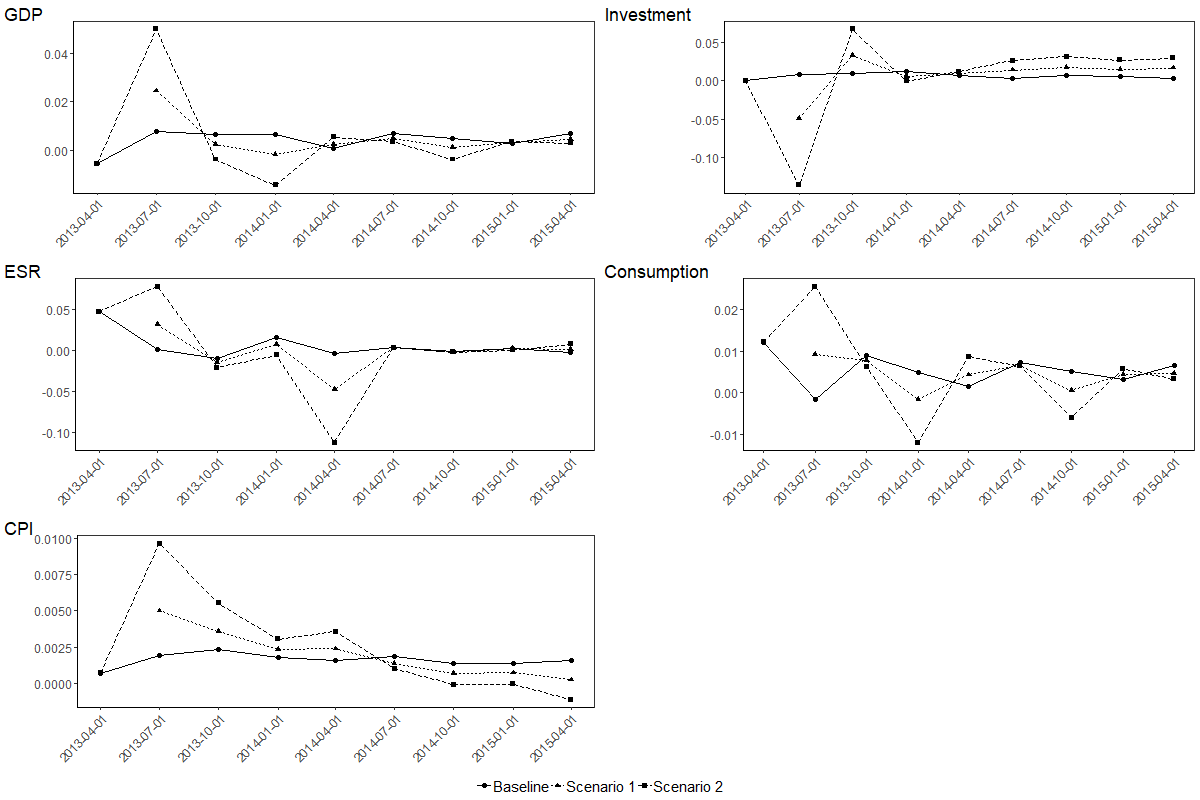
\includegraphics[width=1\textwidth,height=1\textheight,keepaspectratio]{scenariofcst_linearred.png}
	\caption{Forecasts for the policy scenarios for a one-time increase with subsequent gradual reduction.}
	\label{fig:results_dvarLR}
\end{figure} 

\begin{table}[!htbp] \centering 
	\caption{Peak effects and results of Wilcoxon signed-rank test of the scenarios vs baseline for a one-time increase with subsequent gradual reduction.} 
	\label{tab:wtestLR} 
	\begin{tabular}{@{\extracolsep{5pt}} lrrrr} 
		\\[-1.8ex]\hline 
		\hline \\[-1.8ex]
		& Peak Effect 10\% & Peak Effect 25\% & Test Statistic & p \\ 
		\hline \\[-1.8ex] 
		\hline \\[-1.8ex] 
		GDP & $1.69$ p.p. & $4.23$ p.p. & $25$ & $0.38$ \\ 
		Investment & $-5.77$ p.p. & $-14.41$ p.p. & $10$ & $0.31$ \\ 
		ESR & $-4.32$ p.p. & $-10.75$ p.p. & $25$ & $0.38$ \\ 
		Consumption & $-1.09$ p.p. & $2.72$ p.p. & $21$ & $0.74$ \\ 
		CPI & $0.31$ p.p. & $0.77$ p.p. & $15$ & $0.74$ \\ 
		\hline \\[-1.8ex] 
	\end{tabular} 
\end{table}  